\documentclass[]{article}

\usepackage{
	amsmath, 
	amssymb,
	booktabs,
	enumitem,
	float,
	graphicx,
	minted,
	multirow,
	bera,
	parskip
}
\usepackage[table]{xcolor}

\graphicspath{ {Images/} }

\title{Assignment 3}
\author{
	Daniel Bok \\
	ESD \\
	1001049 \\
	daniel\_bok@mymail.sutd.edu.sg 
	\and
	Wong Yan Yee\\ 
	ISTD \\
	1001212 \\
	yanyee\_wong@mymail.sutd.edu.sg
	\and
	Clement Tan \\
	ESD \\
	1000948 \\
	clement\_tan@mymail.sutd.edu.sg
}
\date{\today}

\begin{document}
	
\maketitle

\newpage
\tableofcontents

\newpage
\section{Exercise 1: A Simple Adspace Auction}

\subsection{Bipartite Graph}

\begin{figure}[H]
	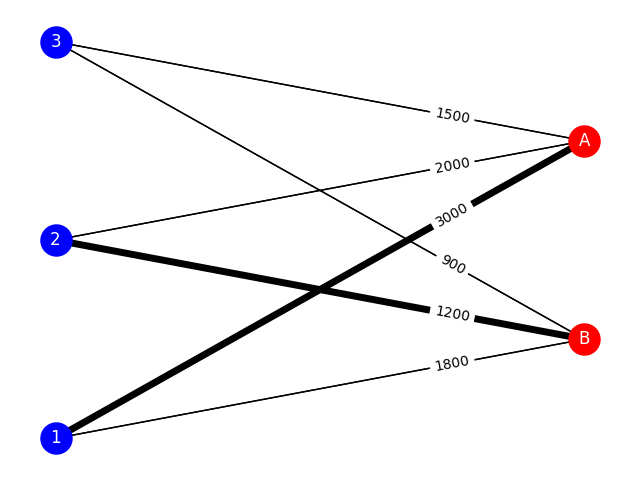
\includegraphics[width=\linewidth]{Image-1.png}
	\caption{Bipartite Graph} 
	\label{Q1.1 Bipartite Graph}
\end{figure}

Figure \ref{Q1.1 Bipartite Graph} above shows the bipartite graph. 

\subsection{Auction Results}

Assuming truthful bidding in the GSP auction, the following outcome happens:

\begin{enumerate}
	\item[\textbf{Allocation}] 
	Advertiser \textbf{1} gets allocated to slot \textbf{A} \\
	Advertiser \textbf{2} gets allocated to slot \textbf{B} \\
	Advertiser \textbf{3} does not get anything
	
	\item[\textbf{Prices}]
	Advertiser \textbf{1} pays \$2000 \\ 
	Advertiser \textbf{2} pays \$900 \\ 
	Advertiser \textbf{3} pays nothing
	
	\item[\textbf{Utility}] 
	Advertiser \textbf{1} gains a utility of \$1000 \\ 
	Advertiser \textbf{2} gains a utility of \$300 \\ 
	Advertiser \textbf{3} gains no (\$0) utility
	
\end{enumerate}

Note that the utility (payoff) is determined by the true valuation of the advertiser and the eventual amount he pays for the slot. If he doesn't get the slot, his utility is 0.


\newpage
\section{eBay Auction}

\begin{table}[htbp]
	\centering
	\caption{Bidding History}
	\begin{tabular}{c|ccccc}
		\rowcolor[rgb]{ 0,  0,  0} \textcolor[rgb]{ 1,  1,  1}{\textbf{Bidders}} & \textcolor[rgb]{ 1,  1,  1}{\textbf{Day 1}} & \textcolor[rgb]{ 1,  1,  1}{\textbf{Day 2}} & \textcolor[rgb]{ 1,  1,  1}{\textbf{Day 3}} & \textcolor[rgb]{ 1,  1,  1}{\textbf{Day 4}} & \textcolor[rgb]{ 1,  1,  1}{\textbf{Day 5}} \\
		\midrule
		\rowcolor[rgb]{ .184,  .459,  .71} \textcolor[rgb]{ 1,  1,  1}{\textbf{1}} & \textcolor[rgb]{ 1,  1,  1}{ \$        7.00 } & \textcolor[rgb]{ 1,  1,  1}{ \$        9.50 } & \textcolor[rgb]{ 1,  1,  1}{ \$     11.00 } & \textcolor[rgb]{ 1,  1,  1}{ - } & \textcolor[rgb]{ 1,  1,  1}{ \$     27.45 } \\
		\rowcolor[rgb]{ .184,  .459,  .71} \textcolor[rgb]{ 1,  1,  1}{\textbf{2}} & \cellcolor[rgb]{ .357,  .608,  .835} \textcolor[rgb]{ 1,  1,  1}{ - } & \textcolor[rgb]{ 1,  1,  1}{ \$        9.25 } & \cellcolor[rgb]{ .357,  .608,  .835} \textcolor[rgb]{ 1,  1,  1}{ - } & \textcolor[rgb]{ 1,  1,  1}{ \$     13.65 } & \cellcolor[rgb]{ .357,  .608,  .835} \textcolor[rgb]{ 1,  1,  1}{ - } \\
		\rowcolor[rgb]{ .184,  .459,  .71} \textcolor[rgb]{ 1,  1,  1}{\textbf{3}} & \textcolor[rgb]{ 1,  1,  1}{ - } & \textcolor[rgb]{ 1,  1,  1}{ - } & \textcolor[rgb]{ 1,  1,  1}{ \$     11.25 } & \textcolor[rgb]{ 1,  1,  1}{ \$     13.90 } & \textcolor[rgb]{ 1,  1,  1}{ \$     17.25 } \\
		\rowcolor[rgb]{ .184,  .459,  .71} \textcolor[rgb]{ 1,  1,  1}{\textbf{Ask Price}} & \cellcolor[rgb]{ .357,  .608,  .835} \textcolor[rgb]{ 1,  1,  1}{ \$        7.25 } & \textcolor[rgb]{ 1,  1,  1}{ \$        9.75 } & \cellcolor[rgb]{ .357,  .608,  .835} \textcolor[rgb]{ 1,  1,  1}{ \$     11.50 } & \textcolor[rgb]{ 1,  1,  1}{ \$     14.15 } & \cellcolor[rgb]{ .357,  .608,  .835} \textcolor[rgb]{ 1,  1,  1}{ \$     17.75 } \\
	\end{tabular}
	\label{Q2.1 Bidding History}
\end{table}

The winning bidder is bidder 1 and she pays \$17.50. We assume that the proxy is done by eBay because it was hinted as such in the text. If that were the case, we thus make the assumption that since eBay knows the maximum limit of the proxy, when someone bids above it, it will automatically use the limit of the proxy as the "second-highest" bid. Thus price paid by the highest bidder will be the "second-highest" bid plus the increment.

\newpage
\section{More Items than Bidders}

We assume that there is a minimum fee $M \geq 0$ to start the bid. We also assume that $b_i$ is bid corresponding to the price that player $i$ is willing to pay for each click on the webpage.

\subsection{Alice's Payoff}

Alice's payoff, $p_1$ is defined by
\begin{align*}
	p_1 = 
	\begin{cases} 
		500(r - b_2) & b1 \geq b2 \qquad  \text{(Case 1)} \\
		300(r - M) & b1 < b2 \qquad \text{(Case 2)}
	\end{cases}
\end{align*}

\subsection{Alice's Optimal Strategy}

Given that this is a Generalized Second-Price (GSP) auction, Alice's dominant strategy is to give a bid equivalent to how much she values the product.

The reason being:
\begin{enumerate}
	\item If Alice bids more than her true value
	\begin{enumerate}[label=\alph*]
		\item Alice's bid exceeds Bob's bid. Alice has to pay Bob's valuation which is higher than her true valuation. Thus her payoff will decrease.
		\item Alice's bid does not exceed Bob's. Alice's payoff remains the same. 
	\end{enumerate}
	\item If Alice bids less than her true value..
	\begin{enumerate}[label=\alph*]
		\item Alice's bid becomes lower than Bob's bid. Alice, instead of winning the bid now loses the bid. Her new payoff now thus decreases.
		\item Alice's bid is still higher than Bob's bid. Alice will still be allocated the same slot and still pay Bob's valuation. Thus her payoff remains the same.
	\end{enumerate}
\end{enumerate}

You see in each of the following situation, if Alice does not bid at her true valuation, she does not get better off, only worse off. Thus the dominant strategy is to bid at her valuation.

\subsection*{In Depth Reason}

If we assume a minimum fixed cost of $M \geq 0$, 2 players and 3 spots, a rational Alice will realize the following.

\begin{enumerate}
	\item She is definitely going to get a slot. The "worst" slot is slot 2
	\item The minimum guaranteed reward she will receive is $P_m = 300(r - M)$, 300 being the click rate of slot 2.
	\item The upper bound for the bid is given by 
	\begin{align*}
		500 (r - T) &= 300(r - M) \\
		T &= r - \frac{3(r - M)}{5}
	\end{align*}
	We will take $T$ to represent her True Bid.
\end{enumerate}

If Alice wants to optimize her profits, she will place a bid of $T$ thus ensuring that $500 (r - T) = 300(r - M)$.

\subsubsection*{Bidding Her True Bid, Alice Wins Slot 1}

Suppose Alice bids greater than her True Bid. Since her bid is still greater than Bob's bid, she will still win that slot and get an effective payout of $500(r - b_2) > 500(r - T) \geq P_m$ since $T > b_2$.

If she lowers her bid, 2 things can happen

\begin{enumerate}
	\item She lowers her bid but her bid is still higher than Bob's. In this case, her payout is still going to be the same.
	\item She lowers her bid and her bid ends up smaller than Bob's.
\end{enumerate}

In the second case, Alice's new payout is $P_m = 300(r - M)$ because she lost the first slot and will get the second slot. However, had her bid been truthful, she would have gotten a payout of $500(r - b_2) > P_m $ since $T > b_2$. Thus in this instance, she will always be better off submitting a truthfully in this first instance.

\subsubsection*{Bidding Her True Bid, Alice Wins Slot 2}

Suppose Alice lowers her bid further. Since her bid is still lower than Bob's bid, she'll still get slot 2 and her effective payout will still be the same. 

If she increases her bid, 2 things can happen

\begin{enumerate}
	\item She increases her bid but her bid is still lower than Bob's.  In this case, her payout is still going to be the same.
	\item She increases her bid and her bid ends up larger than Bob's.
\end{enumerate}

In the second case, Alice's new payout is $500(r - b_2)$. Since we know that $b_2 > T$ and $500(r - b_2) \leq 500(r - T) = P_m$, Alice will thus have a payout lower than $P_m$ which she is guaranteed by submitting her True Bid and getting the second slot.

\newpage
\section{Movie Seats Bidding}
\subsection{SAA without Package Bidding}

If Bidder 1 knew that Bidder 2 will always bid \$10 for one of the seats, Bidder 1 will not bid at all. This is because Bidder 1 with her \$15 budget will never be able to get 2 seats and that getting just a single seat leaves her worse off. Furthermore, if Bidder 1 bids for any 1 seat, Bidder 2 will just bid for the other seat.

Therefore, the outcome can be summarized as follows:
\begin{description}
	\item[Strategy] Bidder 1: No bid. Bidder 2: \$10 for one of either seats.
	\item[Result] Only 1 of the seats is taken by Bidder 2. Bidder 2 only pays \$10 at most for the seat. The other seat will be left empty. 
	\item[Payoffs] Bidder 1 will have no payoff. Bidder 2 will have a payoff equivalent to \$10 minus the price he paid. The theatre will have a payoff equivalent to the price Bidder 2 paid.
\end{description}

\subsection{With Package Bidding}

With the presence of Package Bidding, Bidder 1 can now make a joint bid for the 2 seats at \$15. This is greater than the joint bid of \$12 and individual seat bid of \$10 that Bidder 2 can afford. The theatre will accept Bidder 1's bid as that bid maximizes the overall payoff for the theatre. 

The difference
\begin{enumerate}
	\item Bidder 1 will win
	\item The overall payoff for the theatre increases. From another perspective, this also means that the overall "societal" payoff, increases as more people are happy (Bidder 1 and her husband are happy now).
	\item Bidder 1 can win because her "exposure risk" has decreased with Package Bidding. Exposure Risk refers to the risk of getting an unwanted outcome, namely individual seats in this case, as the bid is all-or-nothing.
\end{enumerate}


\newpage
\section{VCG Auction}

\begin{figure}[H]
	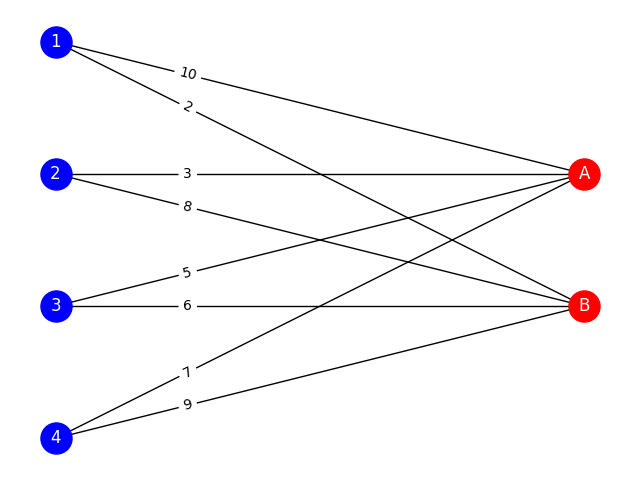
\includegraphics[width=\linewidth]{Image-2.png}
	\caption{Network Graph} 
	\label{Q5.1 Network Graph}
\end{figure}

Figure \ref{Q5.1 Network Graph} above shows the bipartite graph detailing the network relationship. We denote as $v_{ij}$ the value of the edge going from node $i$ to node $j$. In this example, $v_{1A} = 10$. We denote as $B$ the set of all bidders and $I$ the set of all items.

We can apply Integer programming to solve this maximal weighted matching problem with the formula below.

\begin{align*}
	V^* &= \underset{i \in B, j \in I}{\max} \sum c_{ij}v_{ij}\\
	&s.t. \\
	&\sum_{i \in B} c_{ij} \leq 1 \qquad \forall j \in I \\
	&\sum_{j \in I} c_{ij} \leq 1 \qquad \forall i \in B \\
	c_{ij} &= {0, 1}
\end{align*}

The optimal solution to the problem is $V^* = 19$ with $c_{1A} = c_{4B} = 1$. This means Bidder 1 is allocated item A and Bidder 4 is allocated item B.

We denote by $p_{ij}$ the price paid by bidder $i$ for item $j$. The payment by Bidder 1 and 4 is given by

\begin{align*}
	p_{1A} &= V_{\text{no } 1} - \hat{V}_{1 \leftarrow A} \\
		&= (p_{2B} + p_{4A}) - p_{4B} \\
		&= 15 - 9 \\
		&= 6 \\\\
	p_{4B} &= V_{\text{no } 4} - \hat{V}_{4 \leftarrow B} \\
		&= (p_{2B} + p_{1A}) - p_{1A} \\
		&= 18 - 10 \\
		&= 10
\end{align*}


\newpage
\section{Cyclic Ranking}

\begin{gather*}
	\begin{bmatrix}
		0 & 1 & 0 & 0 \\
		0 & 0 & 1 & 0 \\
		0 & 0 & 0 & 1 \\
		1 & 0 & 0 & 0 \\
	\end{bmatrix}
\end{gather*}

As $k$ becomes large, $\pi[k]$ converges to 
\begin{gather*}
	\pi^* = 
	\begin{bmatrix}
		0.5 \\
		0.5 \\
		0 \\
		0
	\end{bmatrix}
\end{gather*}


\newpage
\section{PageRank with different $\theta$}

\begin{enumerate}
	\item[\textbf{0.10}] [ 0.2112  0.2051  0.1999  0.184   0.1999]
	\item[\textbf{0.30}] [ 0.2379  0.223   0.1937  0.1516  0.1937]
	\item[\textbf{0.50}] [ 0.2745  0.2549  0.1765  0.1176  0.1765]
	\item[\textbf{0.85}] [ 0.3941  0.3803  0.0901  0.0453  0.0901]
\end{enumerate}

The bold number of the left represent the value $\theta$ takes and the array on the right represents each webpage's centrality value.

We notice that as $\theta$ increase, PageRank gets better at distinguishing the centrality of each page. This means that the spread between unimportant pages and important pages spread.

Notice the difference between maximum and minimum value at $\theta=0.1$ is 0.0272 while the difference at $\theta=0.85$ is 0.349. This means that PageRank is better at "differentiating" between pages.


\newpage
\section{Block Aggregation in PageRank}

\subsection{PageRank Vector Part 1}

Given:
\begin{align*}
	H &= \begin{bmatrix}
	1 & 0 \\
	\frac{1}{3} & \frac{2}{3}
	\end{bmatrix} \\
\end{align*}

We obtain
\begin{align*}
	G &= 
	\begin{bmatrix}
		0.925 & 0.075 \\
		0.3583 & 0.6417
	\end{bmatrix} \\
	[\pi_A^*, \pi_B^* ] &= 
	\begin{bmatrix}
		0.8269 & 0.1731
	\end{bmatrix}
\end{align*}

\subsection{PageRank Vector Part 2}

The PageRank vectors are given by:
\begin{align*}
	\begin{bmatrix}
		\pi_1^* & \pi_2^*
	\end{bmatrix}^T 
	&=
	\begin{bmatrix}
		0.5 & 0.5
	\end{bmatrix}^T 
	\\
	\begin{bmatrix}
		\pi_3^* & \pi_4^* & \pi_5^*
	\end{bmatrix}^T 
	&=
	\begin{bmatrix}
		0.292 & 0.292 & 0.4161
	\end{bmatrix}^T 
\end{align*}

\subsection{PageRank Vector Part 3}

The approximated PageRank vector is given by:
\begin{align*}
	\tilde{\pi}^* &= \begin{bmatrix}
		\pi^*_A \cdot \begin{bmatrix}
			\pi_1^* & \pi_2^*
		\end{bmatrix}
		&
		\pi^*_B \cdot \begin{bmatrix}
			\pi_3^* & \pi_4^* & \pi_5^*
		\end{bmatrix} 
	\end{bmatrix}^T 
	\\
	&= \begin{bmatrix}
	0.4135 & 0.4135 & 0.0505 & 0.0505 & 0.072
	\end{bmatrix}^T 
\end{align*}

The approximation will increase the computational efficiency in the following ways:
\begin{description}
	\item[\textbf{Memory}] As many parts of the matrix $\mathbf{H}$ will be sparse, this enables clustering of nodes.
	Thus the PageRank algorithm can be run on this smaller clusters (matrices) individually before being aggregated together. The effective memory usage will thus be reduced (we don't need to store many 0s)
	\item[\textbf{Runtime}] The fastest known matrix multiplication runs roughly in $O(N^{2.373})$ time. By reducing the size of the matrix, we effectively reduce the computation runtime. The aggregation operation for the clusters will not affect the runtime much as $c << N$. This constant can be safely ignored in the runtime complexity analysis.
\end{description}

\end{document}
